\documentclass[10pt]{article}
\usepackage{lmodern}
\usepackage[T1]{fontenc}
\usepackage[utf8]{inputenc}
\usepackage{fontspec}
\setmonofont{Source Code Pro}

\newif\ifslow\slowfalse %\slowtrue
\ifslow
  \usepackage[english]{babel}
  \usepackage[babel=true]{microtype}
\fi
\usepackage[top=1in, bottom=1in, left=1.25in, right=1.25in]{geometry}

\usepackage[backend=biber]{biblatex}
\bibliography{bib}

\newcommand{\bdia}{\blacklozenge}
\newcommand{\dia}{\Diamond}
\newcommand{\injR}{\texttt{injR}}
\newcommand{\injL}{\texttt{injL}}


\makeatletter%
\@ifundefined{basedir}{%
\newcommand\basedir{}%
}{}%
\makeatother%
%%%%%%%%%%%%%%%%%%%%%%%%%%%%%%%%%%%%%%%%%%%%%%%%%%%%%%%%%%%%%%%%
%% PACKAGES
%%%%%%%%%%%%%%%%%%%%%%%%%%%%%%%%%%%%%%%%%%%%%%%%%%%%%%%%%%%%%%%%

%\usepackage{amsmath}
\usepackage{amsfonts}
\usepackage{amsthm}
\usepackage{amssymb}
\usepackage{stmaryrd}

\usepackage{\basedir mathpartir}

\usepackage{\basedir pftools}
\usepackage{\basedir iris}

\usepackage{xcolor}  % for print version

\usepackage{graphicx}
\usepackage{enumitem}
\usepackage{semantic}
\usepackage{csquotes}

\usepackage{hyperref}

%%%%%%%%%%%%%%%%%%%%%%%%%%%%%%%%%%%%%%%%%%%%%%%%%%%%%%%%%%%%%%%%
%% SETUP
%%%%%%%%%%%%%%%%%%%%%%%%%%%%%%%%%%%%%%%%%%%%%%%%%%%%%%%%%%%%%%%%
\SetSymbolFont{stmry}{bold}{U}{stmry}{m}{n} % this fixes warnings when \boldsymbol is used with stmaryrd included

\extrarowheight=\jot	% else, arrays are scrunched compared to, say, aligned
\newcolumntype{.}{@{}}
% Array {rMcMl} modifies array {rcl}, putting mathrel-style spacing
% around the centered column. (We used this, for example, in laying
% out some of Iris' axioms. Generally, aligned is simpler but aligned
% does not work in mathpar because \\ inherits mathpar's 2em vskip.)
% The capital M stands for THICKMuskip. The smaller medmuskip would be
% right for mathbin-style spacing.
\newcolumntype{M}{@{\mskip\thickmuskip}}

\definecolor{StringRed}{rgb}{.637,0.082,0.082}
\definecolor{CommentGreen}{rgb}{0.0,0.55,0.3}
\definecolor{KeywordBlue}{rgb}{0.0,0.3,0.55}
\definecolor{LinkColor}{rgb}{0.55,0.0,0.3}
\definecolor{CiteColor}{rgb}{0.55,0.0,0.3}
\definecolor{HighlightColor}{rgb}{0.0,0.0,0.0}

\definecolor{grey}{rgb}{0.5,0.5,0.5}
\definecolor{red}{rgb}{1,0,0}

\hypersetup{%
  linktocpage=true, pdfstartview=FitV,
  breaklinks=true, pageanchor=true, pdfpagemode=UseOutlines,
  plainpages=false, bookmarksnumbered, bookmarksopen=true, bookmarksopenlevel=3,
  hypertexnames=true, pdfhighlight=/O,
  colorlinks=true,linkcolor=LinkColor,citecolor=CiteColor,
  urlcolor=LinkColor
}


%\theoremstyle{definition}
%\newtheorem{prop}{Prop}
\newtheorem{defn}{Definition}
\newtheorem{cor}{Corollary}
\newtheorem{conj}{Conj}
\newtheorem{lem}{Lemma}
\newtheorem{thm}{Theorem}

\newtheorem{exercise}{Exercise}

%%%%%%%%%%%%%%%%%%%%%%%%%%%%%%%%%%%%%%%%%%%%%%%%%%%%%%%%%%%%%%%%
%% GENERIC MACROS
%%%%%%%%%%%%%%%%%%%%%%%%%%%%%%%%%%%%%%%%%%%%%%%%%%%%%%%%%%%%%%%%
\newcommand*{\Sref}[1]{\hyperref[#1]{\S\ref*{#1}}}
\newcommand*{\secref}[1]{\hyperref[#1]{Section~\ref*{#1}}}
\newcommand*{\lemref}[1]{\hyperref[#1]{Lemma~\ref*{#1}}}
\newcommand{\corref}[1]{\hyperref[#1]{Cor.~\ref*{#1}}}
\newcommand*{\defref}[1]{\hyperref[#1]{Definition~\ref*{#1}}}
\newcommand*{\egref}[1]{\hyperref[#1]{Example~\ref*{#1}}}
\newcommand*{\appendixref}[1]{\hyperref[#1]{Appendix~\ref*{#1}}}
\newcommand*{\figref}[1]{\hyperref[#1]{Figure~\ref*{#1}}}
\newcommand*{\tabref}[1]{\hyperref[#1]{Table~\ref*{#1}}}

\newcommand{\changes}{{\bf\color{red}{Changes}}}
\newcommand{\TODO}{\vskip 4pt {\color{red}\bf TODO}}


\newcommand{\ie}{\emph{i.e.,} }
\newcommand{\eg}{\emph{e.g.,} }
\newcommand{\etal}{\emph{et~al.}}
\newcommand{\wrt}{w.r.t.~}

\newcommand{\aaron}[1]{{\color{red}\textbf{AT: #1}}}
\newcommand{\derek}[1]{{\color{red}\textbf{DD: #1}}}
\newcommand{\lars}[1]{{\color{red}\textbf{LB: #1}}}
\newcommand{\kasper}[1]{{\color{red}\textbf{KS: #1}}}
\newcommand{\ralf}[1]{{\color{red}\textbf{RJ: #1}}}
\newcommand{\dave}[1]{{\color{red}\textbf{PDS: #1}}}
\newcommand{\hush}[1]{}
\newcommand{\relaxguys}{%
	\let\aaron\hush%
	\let\derek\hush%
	\let\lars\hush%
	\let\kasper\hush%
	\let\ralf\hush%
	\let\dave\hush%
}


\begin{document}

\title{\bfseries iris-atomic}
\author{Zhen Zhang}
\maketitle

\section{sync.v}

\begin{align}
  \text{synced}(R, f', f) \eqdef
  \All P, Q, x.
    &\hoare{ R * P(x)}{f(x)}{ v.\,R * Q(x,v) } \ra \\
    &\hoare{ P(x)}{f'(x)}{ v.\,Q(x,v) }
\end{align}

Here is the "syncer spec" taken from CaReSL. Note that flat combiner in CaReSL is proven to be contextual refinement of \texttt{mkSync} here, but flat combiner doesn't directly satisfy this spec.

However, there is not program refinement in Iris, so I simply have to prove the flat combiner satisfy exactly this spec directly. This will lead us to a general spec which is not tied to any specific syncer implementation.

\[
  \text{is\_syncer}(R, s) \eqdef
    \All f. \wpre{s(f)}{ f'.\, \text{synced}(R, f', f)} \]


\[
  mk\_syncer\_spec (mk\_syncer) :=
    \All R.
        \hoare{R}{mk\_syncer()}{ s.\,\always (is\_syncer(R, s)} \]

Here is my version, which is approx. splitting the Aaron’s version apart to emphasize the relationship between f and f’. If I use Aaron’s spec, I am afraid I can’t proceed in the first step of synchronization, because f’ is not applied to anything yet!

Another observation is that pre- and post-conditions P, Q are universally qualified per application, that is to say, P, Q is arbitrary, depending on context.

And similarly, f is universally qualified per synchronisation, which means that syncer is only parameterised by the shared resource R, it can work with any operation need to access this R.

The definition below is spec for syncer constructor.

\section{atomic.v}

Logically atomic triple:

\[  
    \lahoare{g.\, \alpha(g)}{e}{v.\, \beta(g, v)}[E_i][E_o] \eqdef
    \All P, Q.
    \begin{aligned}
          &P \vs[Eo][Ei] \Exists g, \alpha(g) * (\alpha(g) \vsW[Ei][Eo] P \land \All v. \beta(g, v) \vsW[Ei][Eo] Q(g, v)) \wand \\
          &\hoare{P}{e}{v.\, \Exists g. Q(g, v)}
    \end{aligned}\]


Okay, now we consider another way of specifying atomicity. This should be familiar to most of you. But here are several things to notice:

1. P Q is arbitrary, depending on context
2. The linear view shift lets us frame some non-persistent context.

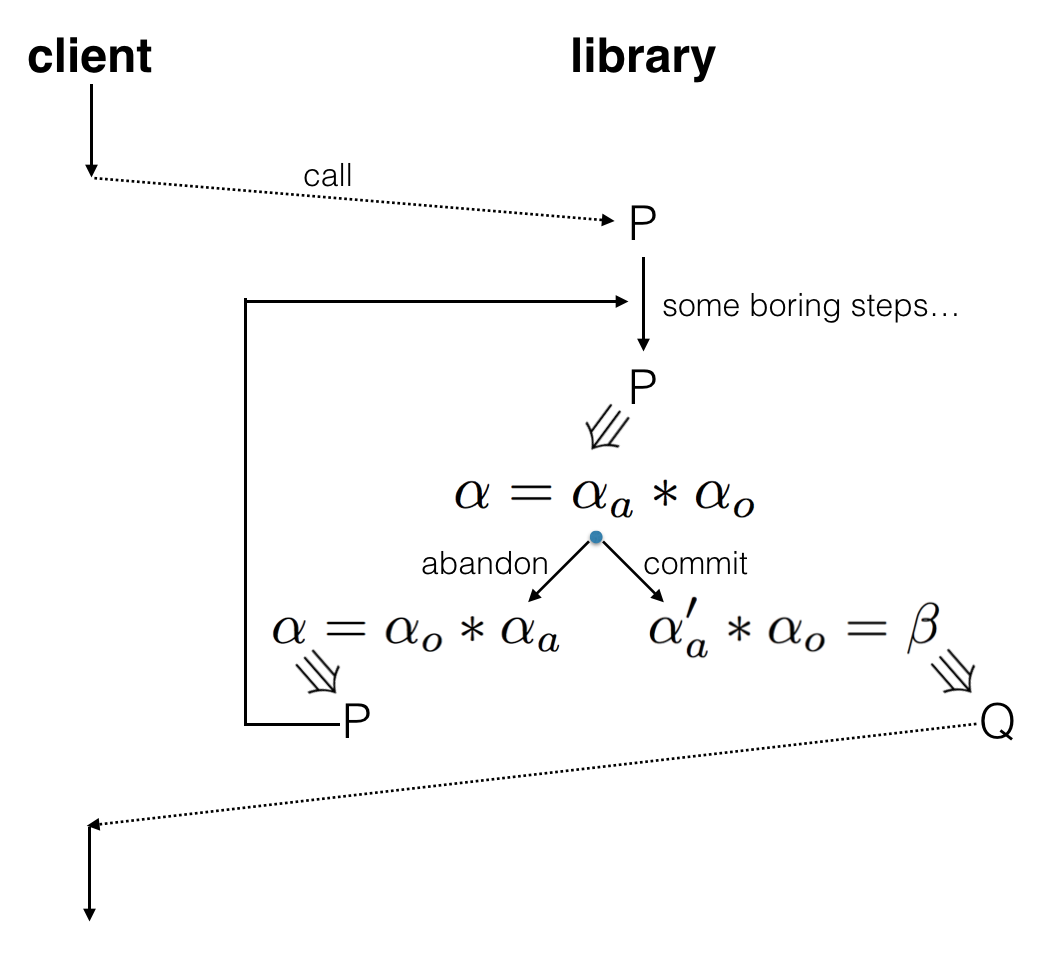
\includegraphics[width=0.5\textwidth]{lat}

Here is a nice picture embodying the central idea … so, now we have introduced two ways of specifying atomicity. I want to give a more high-level picture next

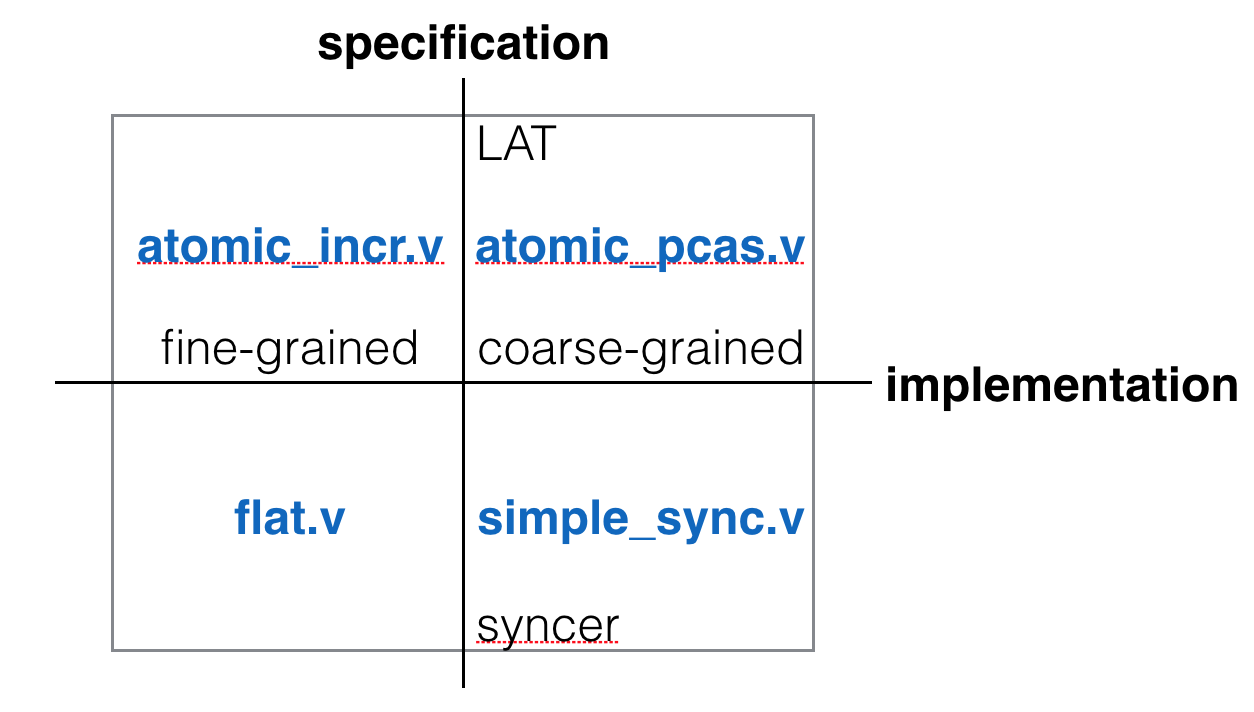
\includegraphics[width=0.5\textwidth]{ispace}

Okay, here is space of my internship…. which has two dimensions.

The vertical dimension is specification, which can either be given like the syncer, or the LAT style spec. The LAT is apparently more general. Actually, we can also feel the same way this from the fact that the atomic triple I derived from syncer spec, is specialised version of general LAT.

Another dimension, the horizontal one, is implementation. We can either use put sequential code inside a pair of lock/unlock, or use some lock-free tricks such as CAS operation or helping to make it fine-grained.

[Special effects]

Okay, here are four proofs which correspond to each facet. Let’s start from \texttt{simple\_sync}.


\section{simple\_sync.v}

\begin{verbatim}
mk_sync :=
    λ: <>,
       let l := newlock() in
       λ: f x,
          acquire l;
          let ret := f x in
          release l;
          ret.
\end{verbatim}

The one on the top is from CaReSL paper, and the one on the bottom is my version written in heap-lang. And fortunately, they are same!

Okay, now the question is: can we give a LAT spec for \texttt{simple\_sync}? Actually, we can, and we can do this in a general way (i.e. not dependent on implementation of syncer).

\section{atomic\_sync.v}

Specialized logically atomic triple:

\[ \lahoare{g.\, \ownGhost{\gname}{g^{1/2}} * \always \alpha(g)}
           {f(x)}
           {v.\, \Exists g'. \ownGhost{\gname}{g'^{1/2}} * \beta(x, g, g', v)}[E_i][E_o]\]

But what kind of LAT do we get from it? How general it is?

Here is what we get. The `g`, ghost state, is of any proper type, and pre-condition alpha is a persistent predicate about state before operation. And in the post condition, we say there exists a ghost state g’ after operation, which satisfy beta , a relation over input, previous state, current state, and output

The \texttt{g\_half} ghost resource is what makes g’ useful. Let’s design the invariant in like this [special effect]. The g in invariant is shared by both physical predicate phi, and the left half of agreement. And by agreeing, we can “synchronize” local ghost state and the global physical state when we open the invariant next time.

\begin{verbatim}
sync(mk_syncer) :=
  λ: f_seq l,
     let s := mk_syncer() in
     s (f_seq l).
\end{verbatim}

\[seq\_spec(f, \phi, \alpha, \beta, E) \eqdef
      \All l.
         \hoare{\top}{f(l)}{f'.\,
            \begin{aligned}
            \pure &\All x, \Phi, g.\\
                &\phi (l, g) * \always \alpha(x) *\\
                &(\All v, g'. \phi(l, g') \wand \beta(x, g, g', v) \wand \pvs[E][E] \Phi(v))\\
                &\proves \wpre{f'(x)}[E]{ \Phi }
              \end{aligned}
        }\]

Here is the sequential spec. pre-condition is the persistent alpha and exclusive ownership of shared state, and when it returns, we got the updated physical state g’, as well as beta.

Funny thing is again that I have to apply f to l first ... because of currying and call site problem.
  
\[\begin{aligned}
      &\text{atomic\_spec}(mk\_syncer, f\_seq, l, \phi, \alpha, \beta, E_i) \eqdef\\
      &\All g_0.
        seq\_spec(f\_seq, \phi, \alpha, \beta, \top) \ra
        mk\_syncer\_spec(mk\_syncer) \ra\\
        &\phi(l, g_0)
        \proves \wpre{sync(mk\_syncer, f\_seq, l)}{ f.\,
          \Exists \gname. \ownGhost{\gname}{g_0^{1/2}} *
          \All x. \always \lahoare{g.\, \ownGhost{\gname}{g^{1/2}} * \always \alpha(g)}{f(x)}
                                  {v.\, \Exists g'. \ownGhost{\gname}{g'^{1/2}} * \beta(x, g, g', v)}[E_i][\top]}
      \end{aligned} \]

So, here is the theorem that states such derivation. Inside the blue box is the triple defined earlier, it is returned in the post-condition.

The meta procedure “sync” is parameterised in Coq with any kind of syncer constructor you want to prove about. Its heap-lang parameters are sequential code closure and the location to internal state. As you can see from its definition, it partially applies \texttt{f\_seq} with l, i.e., binding operation with shared state pointer, and return a concurrent operation synchronized by newly-created syncer.

Now let’s observe its two pure conditions: first, sequential code must have a spec; second, \texttt{mk\_syncer} satisfies the syncer constructor spec [review]

\[ (\Exists g. \phi(l, g') * \ownGhost{\gname}{g^{1/2}} * P x \]

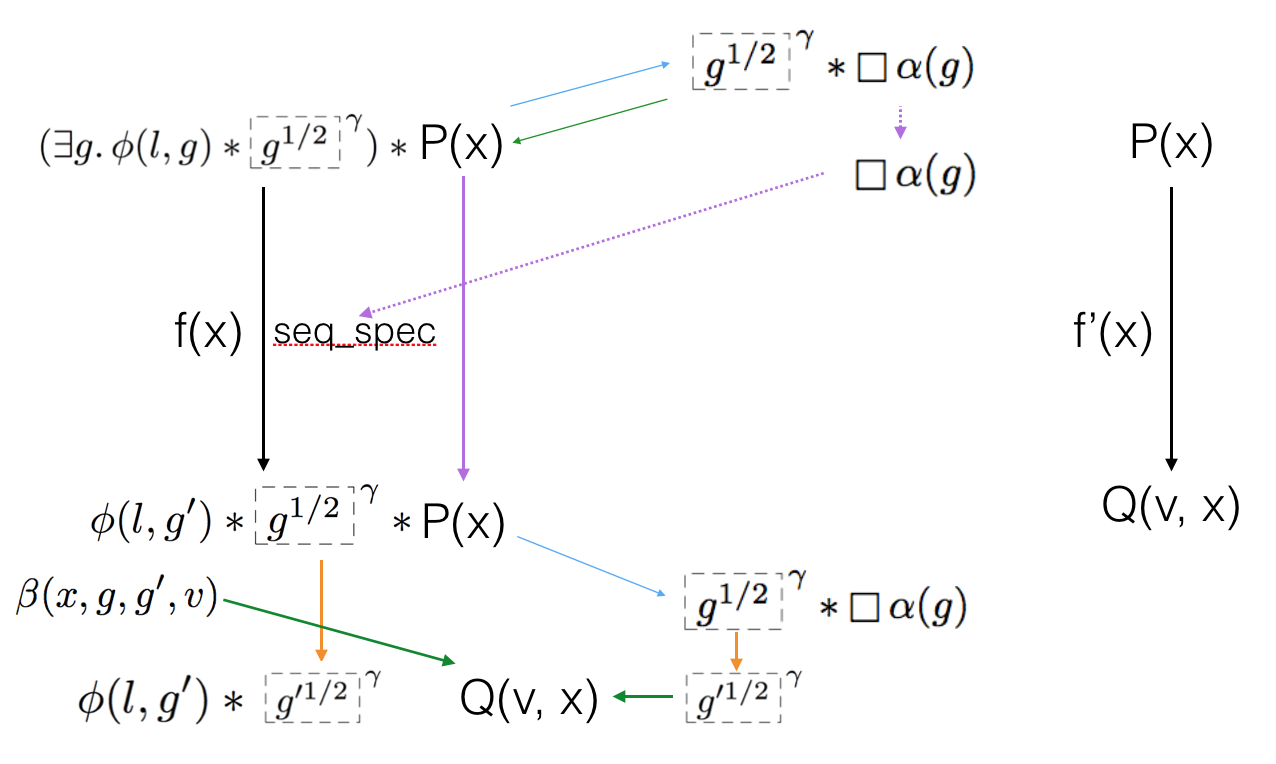
\includegraphics[width=0.5\textwidth]{atomic_sync}

\section{treiber.v}

\begin{verbatim}
push s x :=
  let hd := !s in
  let s' := ref SOME (x, hd) in
  if CAS s hd s'
    then ()
    else push s x.

pop s :=
  let hd := !s in
  match !hd with
  | SOME (x, hd') =>
    if: CAS s hd hd'
      then SOME x
      else pop s
  | NONE => NONE
  end.

iter hd f :=
  match !hd with
  | NONE => ()
  | SOME (x, hd') => f x ; iter hd' f
  end.

\end{verbatim}

Finally, it is time to talk about flat combiner …. oh no, not yet. We need to talk about treiber’s stack first.

These push and pop are all standard lock-free implementation.

We will give LAT spec for these two operations first

Logiall atomic spec (version 1):

\[ \lahoare{xs.\, stack(s, xs)}{push(s, x)}{stack(s, x::xs)}[heapN][\top]\]
\[ \lahoare{xs.\, stack(s, xs)}{pop(s)}{v. \begin{split} (&\Exists x, xs'. v = SOME(x) * stack(s, xs')) \lor\\
                                            (&v = NONE * xs = \emptyset * stack(s, \emptyset)) \end{split}}[heapN][\top]\]


Logiall atomic spec (version 2):

\[ \lahoare{hd, xs.\, s \mapsto hd * list(hd, xs)}{push(s, x)}{\Exists hd'. s \mapsto hd' * hd' \mapsto SOME(x, hd) * list(hd, xs)}[heapN][\top]\]
\[ \lahoare{hd, xs.\, s \mapsto hd * list(hd, xs)}{pop(s)}{v.
    \begin{split}
      (&\Exists x, xs', hd'. v = SOME(x) * hd \mapsto SOME(x, hd') * s \mapsto hd' * list(hd', xs')) \lor\\
      (&v = NONE * xs = \emptyset * hd \mapsto NONE)
    \end{split}
  }[heapN][\top]
  \]

For these two operations, we usually will give a more abstract spec, like the one above, which talks about s and elements in it, but no more.

However, we can also give one that exposes how stack is implemented (here, as a linked list). Actually, if we want to prove push spec in per-item-invariant style, we must expose enough details.

Why? The intuition is that, when push some element in a per-item setting, we need to open, modify where s points to, and then close the invariant. But how can we make sure that the rest of the stack is always satisfying the per-item invariants? If we want such evidence, we need to expose something physical, such as the head pointer in this case.

\section{peritem.v}

A crappy but working spec:

\[f\_spec (\gname, xs, s, f, Rf, RI) \eqdef
    \All x.
      \hoare{x \in xs * \knowInv\iname{\Exists xs. stack'(\gname, xs, s) * RI} * Rf}{f(x)}{ v.\, v = () }.\]

\[\begin{split}
  iter\_spec(\gname, s, Rf, RI) \eqdef
    &\All xs, hd, f.\\
      &f\_spec(xs, s, f', Rf, RI) \ra\\
      &\hoare{\knowInv\iname{\Exists xs. stack'(xs, s) * RI} * list'(\gname, hd, xs) * Rf}{iter(hd, f)}{ v.\, v = () * Rf}
  \end{split}\]

\[push\_spec (\gname, s, x, RI) \eqdef
  \hoare{R(x) * \knowInv\iname{\Exists xs. stack'(xs, s) * RI}}{push(s, x)}{v.\, v = () * (\Exists hd. ev(\gname, hd, x))}\]

Okay, but in per-item spec, why do you need to make sure that the stack is growth-only, and governed by a global invariant?

Answer: because we need to iterate thought it non-atomically. I mean, the process of iteration is not atomic. The single operation f still needs to atomically access any resource related x.

So, having already talked a lot about per-item spec… here is how it looks like in my implementation. Well, I agree with you that this is a bit messy. 

note that global inv of stack is parametrised by per-item predicate R

\section{flat.v}

\begin{verbatim}
doOp :=
  λ: p,
     match !p with
     | InjL (f, x) => p <- InjR (f x)
     | InjR _ => ()
     end.

try_srv :=
  λ: lk s,
    if try_acquire lk
      then let hd := !s in
           iter hd doOp;
           release lk
      else ().

loop p s lk :=
    match !p with
    | InjL _ =>
        try_srv lk s;
        loop p s lk
    | InjR r => r
    end.

install :=
  λ: f x s,
     let p := ref (InjL (f, x)) in
     push s p;
     p.

mk_flat :=
  λ: <>,
   let lk := newlock() in
   let s := new_stack() in
   λ: f x,
      let p := install f x s in
      let r := loop p s lk in
      r.
\end{verbatim}


Let’s go to my flat combiner code now.

Compared to CaReSL, here are several notable differences:

I break them down into five procedures, instead of nesting them inside the constructor. It is easier to specify.
CaReSL’s flat constructor takes f; this doesn’t, which makes it more flexible.
CaReSL’s install utilize TLS to avoid blowup of space use. I push in a new slot every time, which is terrible in practice, but follows the same spec.

Also, another problem that exist both in my, CaReSL, and FCSL’s example code, is that we never recycle the slots.

\[p \mapsto \injR(-)\]
\[p \mapsto \texttt{injL}(f, x)\]
\[p \mapsto \injR(y)\]
\[\circ_i, \bullet_i, \dia_i, \bdia, \dia_i \circ_i, \dia_i \bullet_i, \bdia \bullet_i\]


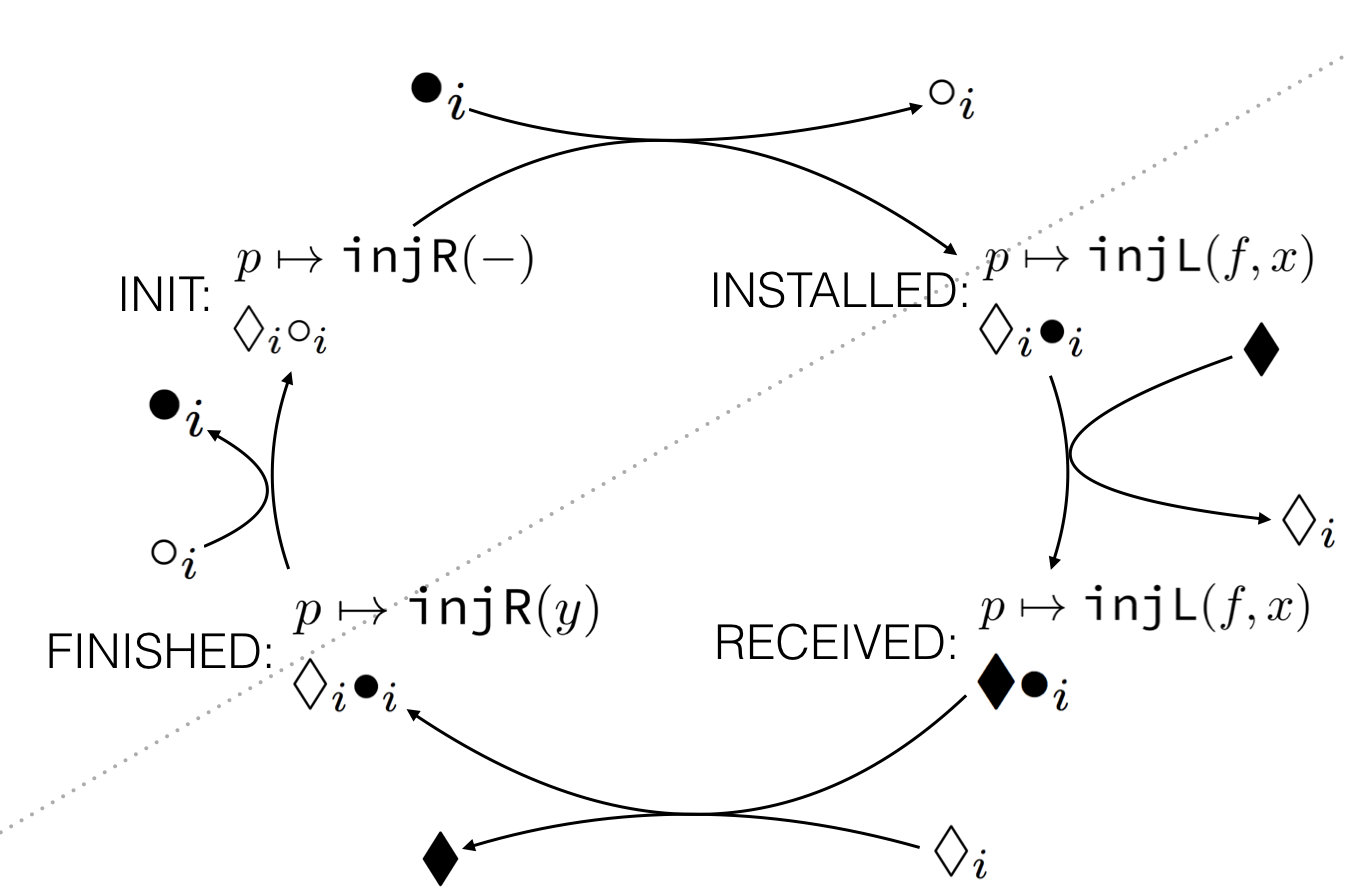
\includegraphics[width=0.5\textwidth]{helping}

This is the protocol of helping … 

The black diamond is a token owned by server lock.
The other three kinds of token are all tagged with i, which should be similar to thread id in CaReSL’s reasoning, but in my case, it is the slot address (Is it more flexible than using tid to index?). And the indexing is essentially done through a ghost map in invariant. 

Note that this graph is heavily simplified to reflect how I encode protocol with bare exclusive monoids. Next slide gives the detailed invariant construction


\begin{align*}
     &\Exists y.          &&p \fmapsto[1/2] \injR(-) * \dia_i * \circ_i\\
\lor &\Exists f, x, P, Q. &&p \fmapsto[1/2] \injL(f, x) * \ownGhost{\gname}{x^{1/2}} *
                           P(x) * (\hoare{R * P(x)}{f(x)}{v.\,R * Q(x, v)}) * \gamma \mapstoprop Q(x) * \dia_i * \bullet_i\\
\lor &\Exists x.          &&p \fmapsto[1/2] \injL(-, x) * \ownGhost{\gname}{x^{1/4}} * \bdia * \bullet_i\\
\lor &\Exists x, y.       &&p \fmapsto[1/2] \injR(y) * \ownGhost{\gname}{x^{1/2}} * \gamma \mapstoprop Q(x) * Q(x, y) * \dia_i * \bullet_i
\end{align*}

Here is the per-item (i.e. request slot) invariant, which have four branches.

Note how f x P Q are all hidden under existential qualification, while (Q x) is saved under some name. It means that only post-condition matter to waiting client.

This is basically the core of flat combiner proofs. There are just a couple of critical points, the rest are all boilerplates like open/close invariant. A nicer per-item spec could improve it I guess.

\[\alpha = \alpha_a * \alpha_o, \alpha = \alpha_a' * \alpha_o\]
\[\alpha = \alpha_o * \alpha_a, \alpha_a' * \alpha_o = \beta\]
\[\alpha = \alpha_a * \alpha_o, \alpha = \alpha_a' * \alpha_o\]

\end{document}
